\documentclass[9pt,a4paper]{extarticle}
\usepackage[margin=2cm]{geometry}
\usepackage{amsmath,amssymb,booktabs,graphicx,microtype,float}
\usepackage[colorlinks=true,urlcolor=blue,linkcolor=black]{hyperref}
\title{Hybrid MPI--OpenMP K-means Clustering:\\Implementation, Validation, and Scaling}
\author{DSA5208 Project 3\\[0.5em]Zimo Xia\\Yixiao Xu}
\date{29 October 2026}
\begin{document}
\maketitle
\begin{abstract}
We implement Lloyd's K-means in C++17 with MPI observation partitioning and OpenMP thread parallelism. Thread-private sufficient statistics avoid races; MPI collectives synchronize centroid updates. An independent serial implementation verifies correctness. On an eight-core laptop, 15 iterations on one million 32-dimensional observations and 16 clusters achieve a 4.39-fold speedup with eight workers. On the NUS Atlas 8 cluster, 24 workers across two nodes achieve a 17.91-fold speedup, while six-process weak-scaling efficiency is 95.7\%. Source, raw measurements, and a benchmark driver accompany this report.
\end{abstract}

\section{Algorithm and data}
For observations $x_i\in\mathbb{R}^D$ and centroids $\mu_c$, K-means minimizes
\begin{equation}
J=\sum_{i=1}^{N}\min_{1\leq c\leq K}\lVert x_i-\mu_c\rVert_2^2.
\end{equation}
Lloyd's procedure alternates nearest-centroid assignment with replacing each centroid by the mean of its assigned observations \cite{lloyd}. We run a fixed number of iterations to make scaling measurements comparable. Empty clusters retain their previous centroids, and ties use the lowest centroid index. Assignment dominates at $O(NKD)$ operations per iteration.

The controlled synthetic dataset is deterministic across process counts. Observation $i$ has generating group $i\bmod K$. Its first coordinate is $3(i\bmod K)$ plus uniform noise in $[-1,1)$; other coordinates use a smaller group-dependent offset and independent noise. A 64-bit hash of global observation index, dimension, and seed generates each value. The first $K$ observations initialize the centroids. This is a computational benchmark rather than an analysis of real data.

\section{Parallel design}
MPI partitions contiguous global observation indices among $P$ processes, distributing remainders to the lowest ranks. Each process generates only its own data, requiring $O(ND/P)$ observation storage and no scatter. All ranks independently generate the same initial centroids. Within a rank, an OpenMP static loop processes observations. Each of $T$ threads owns a private $K\times D$ sum matrix and $K$ counts, using $O(TKD)$ additional storage but avoiding atomics. After local combination, two \texttt{MPI\_Allreduce} calls sum the process statistics. Each process then makes the same centroid update. MPI is called outside the parallel region under \texttt{MPI\_THREAD\_FUNNELED}. Two collective synchronizations occur per iteration. Floating-point summation order varies with worker count, so bitwise identical centroids are not expected.

\section{Validation and experiment}
An independent serial reference regenerates all points and repeats the assignment and update. Validation fails if any final centroid differs by more than $10^{-8}$. An uneven partition ($N=4001,D=5,K=4$, two MPI processes, two threads) had maximum difference $8.88\times10^{-15}$. A one-cluster case ($N=17,D=1,K=1$, four processes) agreed exactly. The strong-scaling runs all produced final inertia 10,666,433.79 and 99.993\% agreement with known generating labels to displayed precision. Label agreement is a synthetic-data diagnostic, not an out-of-sample accuracy measure.

Runs used a MacBookPro18,3 with eight physical/logical CPU cores, 32 GiB memory, macOS 26.6.2, Open MPI 5.0.11, and GCC 16.2.0 with \texttt{-O3 -std=c++17 -fopenmp}. Each configuration was repeated five times; tables give medians and full ranges. Timing begins after data generation and an MPI barrier and ends after 15 assignment/update iterations. It includes computation and collectives but excludes process launch, data generation, and final quality calculations. The maximum rank time measures whole-job completion. Strong scaling holds $N=10^6,D=32,K=16$ fixed. Weak scaling holds 250,000 points per MPI process and one thread per process. Dynamic OpenMP team sizing was disabled. All tests ran on one machine.

\section{Scaling results}
Strong speedup is $S_p=T_1/T_p$ and efficiency is $S_p/p$, where $p$ counts all process--thread workers. Weak efficiency is baseline time divided by time with $P$ processes and $P$ times the dataset size.
\begin{table}[H]\centering\small
\caption{Strong scaling, $N=1000000$, $D=32$, $K=16$, 15 iterations. Times are medians of 5 runs; ranges show minimum and maximum.}
\begin{tabular}{rrrrrrr}\toprule
MPI & OMP & Workers & Time (s) & Range (s) & Speedup & Efficiency \\
\midrule
1 & 1 & 1 & 4.481 & 4.472--4.497 & 1.00 & 100.0\% \\
1 & 2 & 2 & 2.274 & 2.247--2.296 & 1.97 & 98.5\% \\
1 & 4 & 4 & 1.179 & 1.156--1.214 & 3.80 & 95.0\% \\
1 & 8 & 8 & 1.089 & 1.021--1.228 & 4.11 & 51.4\% \\
2 & 1 & 2 & 2.404 & 2.280--2.603 & 1.86 & 93.2\% \\
4 & 1 & 4 & 1.281 & 1.252--1.518 & 3.50 & 87.5\% \\
2 & 2 & 4 & 1.297 & 1.267--1.429 & 3.45 & 86.4\% \\
4 & 2 & 8 & 1.022 & 0.980--1.100 & 4.39 & 54.8\% \\
\bottomrule\end{tabular}\label{tab:strong}\end{table}
\begin{table}[H]\centering\small
\caption{Weak scaling with 250,000 observations per MPI process and one OpenMP thread.}
\begin{tabular}{rrrrr}\toprule
MPI & Observations & Time (s) & Range (s) & Weak efficiency \\
\midrule
1 & 250,000 & 1.141 & 1.109--1.164 & 100.0\% \\
2 & 500,000 & 1.172 & 1.150--1.196 & 97.4\% \\
4 & 1,000,000 & 1.295 & 1.227--2.095 & 88.1\% \\
\bottomrule\end{tabular}\label{tab:weak}\end{table}

\begin{figure}[H]
\centering
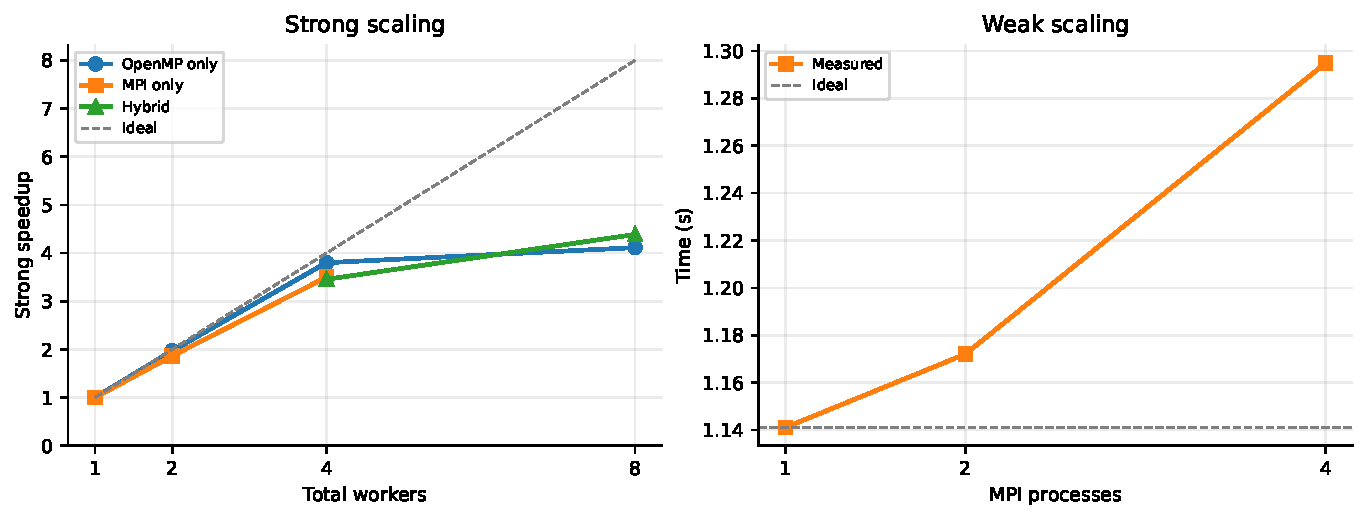
\includegraphics[width=0.88\linewidth]{scaling.pdf}
\caption{Measured strong speedup and weak-scaling time. Dashed lines represent ideal scaling.}
\end{figure}

Four OpenMP threads reached 3.80-fold speedup and 95.0\% efficiency; eight threads reached 4.11-fold and 51.4\%. Memory bandwidth pressure and thread overhead are possible explanations, but neither was measured separately. With four total workers, four MPI processes achieved 3.50-fold and two processes with two threads each achieved 3.45-fold; one process with four threads was faster. The fastest configuration was four processes with two threads each: 1.022 seconds and 4.39-fold speedup. Median collective time there was 0.113 seconds, about 11.1\% of total time, including synchronization waits.

Weak-scaling median time increased from 1.141 seconds at one process to 1.172 at two and 1.295 at four. Efficiency was 97.4\% and 88.1\%, respectively. The four-process runs varied from 1.227 to 2.095 seconds, showing local runtime noise. The displayed strong-scaling inertia and label agreement were unchanged across configurations.

\section{Atlas 8 cluster experiment}
We repeated the same fixed workload on NUS Atlas 8 under PBS, requesting two nodes with 12 CPUs on each node. Each node hosted three MPI processes with four OpenMP threads in the largest configuration. A six-process placement check recorded three processes on each of \texttt{cnode-33-43-34} and \texttt{cnode-33-43-46}. The job loaded GCC 13.2.0, Open MPI 4.1.6, and Python 3.11.5; compilation used the same \texttt{-O3} and OpenMP flags. Open MPI used PBS's \texttt{pbs\_tmrsh} launch agent and no process binding. The cluster executable passed both serial-reference validation cases before measurement. Five repetitions per configuration used $N=10^6,D=32,K=16$ and 15 iterations for strong scaling, and 250,000 observations per process with one thread per process for weak scaling. Timing boundaries match the laptop runs.

\begin{table}[H]\centering\small
\caption{Strong scaling, $N=1000000$, $D=32$, $K=16$, 15 iterations. Times are medians of 5 runs; ranges show minimum and maximum.}
\begin{tabular}{rrrrrrr}\toprule
MPI & OMP & Workers & Time (s) & Range (s) & Speedup & Efficiency \\
\midrule
1 & 1 & 1 & 4.096 & 4.092--4.146 & 1.00 & 100.0\% \\
1 & 4 & 4 & 1.064 & 1.025--1.095 & 3.85 & 96.2\% \\
2 & 4 & 8 & 0.559 & 0.548--0.574 & 7.32 & 91.5\% \\
3 & 4 & 12 & 0.395 & 0.393--0.421 & 10.38 & 86.5\% \\
6 & 4 & 24 & 0.229 & 0.215--0.378 & 17.91 & 74.6\% \\
\bottomrule\end{tabular}\label{tab:hpc-strong}\end{table}
\begin{table}[H]\centering\small
\caption{Weak scaling with 250,000 observations per MPI process and one OpenMP thread.}
\begin{tabular}{rrrrr}\toprule
MPI & Observations & Time (s) & Range (s) & Weak efficiency \\
\midrule
1 & 250,000 & 1.010 & 1.008--1.015 & 100.0\% \\
2 & 500,000 & 1.020 & 1.017--1.024 & 99.0\% \\
3 & 750,000 & 1.023 & 1.021--1.050 & 98.7\% \\
6 & 1,500,000 & 1.055 & 1.043--1.062 & 95.7\% \\
\bottomrule\end{tabular}\label{tab:hpc-weak}\end{table}

\begin{figure}[H]
\centering
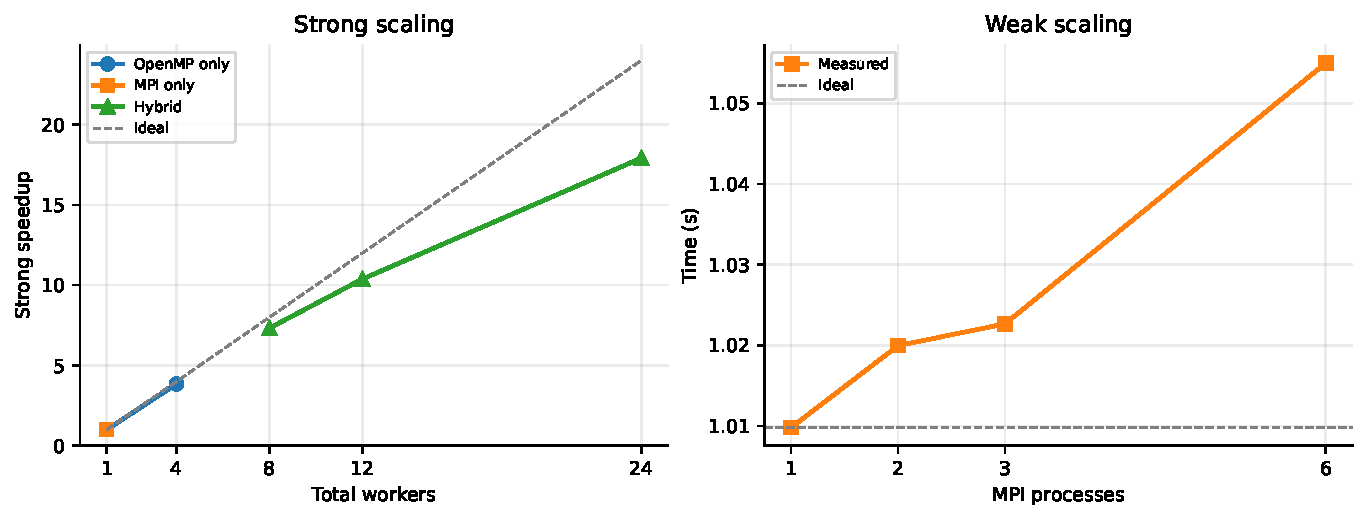
\includegraphics[width=0.88\linewidth]{hpc/scaling.pdf}
\caption{Atlas 8 strong speedup and weak-scaling time. The 24-worker strong run and six-process weak run span two nodes.}
\end{figure}

The two-node 6-process, 4-thread run took a median 0.229 seconds, 17.91 times faster than the 4.096-second cluster serial baseline, with 74.6\% efficiency across 24 workers. The range was 0.215--0.378 seconds, wider than at lower worker counts. Median collective time rose from approximately 0.0001 seconds at one process to 0.050 seconds at six processes, about 22\% of the 24-worker elapsed time. This includes waiting at collectives, so it cannot be attributed entirely to network transfer. Weak-scaling time increased from 1.010 to 1.055 seconds as the dataset grew sixfold, yielding 95.7\% efficiency. Strong-run inertia remained 10,666,433.79 at displayed precision across configurations. A separate 12-CPU, one-node PBS run completed 35 measurements and found 0.401 seconds for three processes with four threads, close to the 0.395-second median in the two-node allocation; its raw data are included for comparison.

\section{Convergence and cost analysis}
The fixed 15-iteration budget exceeds the number of iterations needed for the synthetic dataset to stabilize. A separate $N=200{,}000$, $D=32$, $K=16$ experiment with two MPI processes and two threads per process recorded the final objective after selected iteration counts:
\begin{table}[H]\centering\small
\caption{Final inertia and generating-label agreement by iteration count.}
\begin{tabular}{rrr}\toprule
Iterations & Inertia & Label agreement \\
\midrule
1 & 2,146,785.98 & 99.9790\% \\
2 & 2,134,374.87 & 99.9955\% \\
5 & 2,134,374.51 & 99.9950\% \\
15 & 2,134,374.51 & 99.9950\% \\
\bottomrule\end{tabular}\end{table}
The objective is non-increasing in these measurements and is unchanged to two decimal places between five and 15 iterations. Label agreement can fluctuate slightly even as inertia improves, because the K-means objective is squared distance, not recovery of generating labels. The 15-iteration setting intentionally measures a fixed workload rather than an early-stop implementation.

Per-iteration assignment cost falls roughly as $NKD/(PT)$ when observations divide evenly, but this approximation omits memory traffic, scheduling, and two global reductions. Local data, thread-private sums, centroid storage, and local/global reduction buffers require approximately $8ND/P+8(T+3)KD$ bytes, plus count and control arrays. For the one-million-point strong-scaling case, the observation array alone occupies about 256 MB at one process or 64 MB per process at four processes. Increasing process count reduces this local array but adds collective synchronization, consistent with the larger communication fractions and the decline in efficiency at eight workers. These observations explain the measured trends without claiming a fitted hardware performance model.

\section{Limitations and conclusion}
The clusters are well separated and do not test difficult initialization or imbalance. Fixed iterations omit convergence stopping. The timings cover the iterative kernel, not end-to-end data generation. The two-node experiment establishes performance for this workload and allocation, but does not characterize larger node counts or other datasets. More difficult data and broader cluster allocations would test generality. Within the tested settings, the hybrid implementation agrees with the serial reference and scales to 24 workers across two nodes.

\section{Reproducibility}
The implementation, serial validator, measurement driver, and figure generator are included with this report. The source is built with the supplied Makefile. On a system with Open MPI, a GNU C++ compiler, and Python with Matplotlib, the following commands reproduce the validation and performance study from the project root:
\begin{verbatim}
make CXX=/path/to/g++
make check
python3 benchmark.py --repetitions 5
python3 make_figures.py
\end{verbatim}
The driver writes individual measurements, summary statistics, and machine information to the \texttt{results} directory as \texttt{raw.jsonl}, \texttt{summary.csv}, and \texttt{machine.json}. It executes the eight laptop strong-scaling configurations in Table~\ref{tab:strong} and the three laptop weak-scaling configurations in Table~\ref{tab:weak}. The figure and tables are generated directly from the summary CSV, avoiding manual transfer of measured times.

On Atlas 8, submit \texttt{qsub hpc/atlas8.pbs} from the project root. The PBS script requests two nodes, records node and rank placement, rebuilds and validates the executable, and writes 45 individual measurements plus summaries to \texttt{results/hpc-atlas8}. The companion \texttt{hpc/atlas8-one-node.pbs} records 35 one-node measurements in its own directory. To regenerate the cluster table and plot, run \texttt{python3 make\_figures.py --summary results/hpc-atlas8/summary.csv --output-dir report/hpc --label-prefix hpc-}.

The seed defaults to 5208. For other problem sizes, the executable accepts \texttt{--n}, \texttt{--d}, \texttt{--k}, \texttt{--iterations}, and \texttt{--seed}. The \texttt{OMP\_NUM\_THREADS} environment variable and \texttt{mpirun -np} argument select the two parallel dimensions.

\section*{AI usage disclosure}
The code for this project was generated using AI. The project structure was designed by the group members. The group members reviewed and checked the AI-generated code and take responsibility for the final submission.

\begin{thebibliography}{9}
\bibitem{lloyd} S. P. Lloyd, Least squares quantization in PCM, \emph{IEEE Transactions on Information Theory}, 28(2), 129--137, 1982. \url{https://doi.org/10.1109/TIT.1982.1056489}.
\bibitem{mpi} MPI Forum, \emph{MPI Documents}. \url{https://www.mpi-forum.org/docs/}.
\bibitem{openmp} OpenMP Architecture Review Board, \emph{OpenMP API Specifications}. \url{https://www.openmp.org/specifications/}.
\end{thebibliography}
\end{document}
